
With this background Buchberger's summary statement, "Mathematica implements - as part of its basic language interpreter - an evaluator for higher order conditional rewriting," \cite[p. 8]{buchberger_mathematica_1996} can be understood, if evaluation and higher order are given their dues as well. 

Rewriting is performed until no further rewriting is possible but is dependent on specificity of the rule, as explored further in Section \ref{symbolic-expressions}: the order in which this happens is implemented in the evaluator, described in the original software documentation for the system - As a note on Mathematica/Wolfram Language documentation at this point: Bruno Buchberger references the companion book for Version 3.0 of Mathematica \cite{noauthor_wolfram_nodate}, available online - "The Documentation Center’s fundamental material was based on Stephen Wolfram’s The Mathematica Book, and Stephen Wolfram continues to be responsible for the core reference documentation for Mathematica." \cite{noauthor_mathematica_nodate}

Still concerned with evaluation in Wolfram Language in general, and Mathematica Version 3.0 in the present line of inquiry, and drawing on the availability of legacy documentation, it make sense to contrast The Mathematica Book as Buchberger wrote to with that of Version 14.0, the current version, to test the stability of these fundamental concepts. Buchberger references this part of the documentation concerned with expressions, evaluation and evaluation order - covering the basics we have concerned ourselves with so far:

\begin{displayquote}
The fundamental operation that Mathematica performs is evaluation. Whenever you enter an expression, Mathematica evaluates the expression, then returns the result. 
Evaluation in Mathematica works by applying a sequence of definitions. The definitions can either be ones you explicitly entered, or ones that are built into Mathematica. 
Thus, for example, Mathematica evaluates the expression 6+7 using a built-in procedure for adding integers. Similarly, Mathematica evaluates the algebraic expression x-3x+1 using a built-in simplification procedure. If you had made the definition x=5, then Mathematica would use this definition to reduce x-3x+1 to -9. 
The two most central concepts in Mathematica are probably expressions and evaluation.
\cite[2.5.1 Principles of Evaluation]{noauthor_wolfram_nodate}
\end{displayquote}

The Mathematica Book goes on the define the Standard Evaluation Procedure that applies to Buchberger's discussion at the time:

\begin{displayquote}
\begin{itemize}
    \item Evaluate the head of the expression.
    \item Evaluate each element in turn.
    \item Apply transformations associated with the attributes Orderless, Listable and Flat.
    \item Apply any definitions that you have given.
    \item Apply any built-in definitions.
    \item Evaluate the result.
\end{itemize}
\cite[2.5.4 The Standard Evaluation Procedure]{noauthor_wolfram_nodate}
\end{displayquote}

Most crucially, and this correlates with the central, recursive and repeated, rewriting idea as presented by Buchberger:

\begin{displayquote}
As discussed in Section 2.5.1, Mathematica follows the principle that each expression is evaluated until no further definitions apply. This means that Mathematica must continue re-evaluating results until it gets an expression which remains unchanged through the evaluation procedure.
\cite[2.5.4 The Standard Evaluation Procedure]{noauthor_wolfram_nodate}
\end{displayquote}

(This is what rewriting is about: the Mathematica documentation puts in the terms Wolfram Research finds for the process in the context of its system. Notes such as implementation details relating to the stack used in evaluations are also already present for Mathematica Version 3.0. \cite{noauthor_wolfram_nodate})

Contrast this to current documentation: The central procedure (sequence) is similar, but has become more complex. We consider an expression \(h[e1,e2…]\). ("Every time the expression changes, the Wolfram Language effectively starts the evaluation sequence over again." \cite{noauthor_evaluationwolfram_nodate})

\begin{displayquote}
\begin{itemize}
    \item If the expression is a raw object (e.g., Integer, String, etc.), leave it unchanged.
    \item Evaluate the head \(h\) of the expression.
    \item Evaluate each element \(e_i\) of the expression in turn. If \(h\) is a symbol with attributes HoldFirst, HoldRest, HoldAll, or HoldAllComplete, then skip evaluation of certain elements.
    \item Unless \(h\) has attributes SequenceHold or HoldAllComplete, flatten out all Sequence objects that appear among the \(e_i\).
    \item Unless \(h\) has attributes SequenceHold or HoldAllComplete, flatten out all Sequence objects that appear among the \(e_i\).
    \item Unless \(h\) has attribute HoldAllComplete, strip the outermost of any Unevaluated wrappers that appear among the \(e_i\).
    \item Unless \(h\) has attribute HoldAllComplete, strip the outermost of any Unevaluated wrappers that appear among the \(e_i\).
    \item If \(h\) has attribute Flat, then flatten out all nested expressions with head \(h\).
    \item If \(h\) has attribute Listable, then thread through any \(e_i\) that are lists.
    \item If \(h\) has attribute Orderless, then sort the \(e_i\) into order.
    \item Unless \(h\) has attribute HoldAllComplete, use any applicable transformation rules associated with \(f\) that you have defined for objects of the form \(h[f[e1,…],…]\).
    \item Use any built‐in transformation rules associated with \(f\) for objects of the form \(h[f[e1,…],…]\).
    \item Use any applicable transformation rules that you have defined for \(h[f[e1,e2,…],…]\) or for \(h[…][…]\).
    \item Use any built‐in transformation rules for \(h[e1,e2,…]\) or for \(h[…][…]\).
\end{itemize}
\cite[The Standard Evaluation Sequence]{noauthor_evaluationwolfram_nodate}
\end{displayquote}

One of the more concrete changes in this historical view is the possibility for controlling the evaluation sequence with WL-options \cite{noauthor_optionswolfram_nodate}, for "holding" evaluations. This sequence implements the basic evaluation logic underlying the Mathematica system in this way: Interesting to note in these documentation excerpts is the doubling of expressions as objects, an essential conceptual component explored in Section \ref{oop}.

Buchberger specifies rewriting in Mathematica as higher order conditional rewriting: we have already seen how WL as a rewriting language is one in which computation is performed by repeatedly applying rules to transform expressions into different forms. Adding a layer of logic and control over how expressions are transformed, making the rewriting process more powerful and flexible, is what conditions achieve. In this context, "higher-order" refers to the ability of WL to manipulate not just values but also functions and rules themselves. In Mathematica, function- and rule-expressions can be passed as arguments, returned as values, and stored in data structures. Program \ref{higherorder} is a code example with comments that demonstrates these capabilities succinctly.

\begin{program}
\caption{A rule and its application in WL: \lstinline*rule = x_ /; x > 10 :> x^2;* defines a rule named rule that applies to any expression matching \lstinline*x_* (which represents any expression) but only if the condition \lstinline*x > 10* is true. If the condition is met, the expression \lstinline*x* is transformed to \lstinline*x^2*.}
\label{higherorder}
\begin{LaTeXCode}
(* Define a rule that squares a number if it's greater than 10 *)
rule = x_ /; x > 10 :> x^2;

(* Apply the rule to a list of numbers *)
{5, 10, 15, 20, 25} /. rule

(*

Here's what happens to each element as the rule is applied, using "/.":

* 5 does not meet the condition (5 > 10 is false), so it remains 5.
* 10 does not meet the condition (10 > 10 is false), so it remains 10.
* 15 meets the condition (15 > 10 is true), so it is squared to become 225.
* 20 meets the condition (20 > 10 is true), so it is squared to become 400.
* 25 meets the condition (25 > 10 is true), so it is squared to become 625.

*)
\end{LaTeXCode}
\end{program}

Some WL shorthand notation was used here: Together with pure functions (also known as (pure) anonymous functions), the technical specifics need to be passed over for the sake of brevity at this point, apart from the following helpful "Tech Note" relating these terms to the functional programming paradigm (see Section \ref{high-level}), as a preview of where to go next from rewriting, in discussing relevant theory (Chapter \ref{cha:Theory}), and as a note on the sometimes imprecise language involved.

\begin{displayquote}
Pure functions are a characteristic feature of functional programming. They’re often called lambda expressions, after their use in mathematical logic in the 1930s. Confusingly, the term “pure function” sometimes just means a function that has no side effects (i.e. assigns no values to variables, etc.)
\cite[First note in Tech Notes]{noauthor_pure_nodate}
\end{displayquote}

To not jump ahead however, let us backtrack and take a look at the simple example of a named function and its pure correlate, using the \lstinline+#+ (slot for the variable) and \lstinline+&+ (end of the pure function) notation available in WL, in Program \ref{purefnwithshorthand} taken from \cite{noauthor_functional_nodate}.

\begin{program}
\caption{From \cite{noauthor_functional_nodate}, this example demonstrates the use of the higher order Map \cite{noauthor_map_nodate} both with a named function and its unnamed, "pure" version.}
\label{purefnwithshorthand}
\begin{LaTeXCode}
h[x_] := f[x] + g[x] (* named function *)
Map[h, {a, b, c}] (* using the name in Map, a higher order function *)
Map[f[#] + g[#] &, {a, b, c}] (* the pure function correlate of the previous line *)
\end{LaTeXCode}
\end{program}

The named version makes it easier to see how in an expression like h[x], the "function name" h is of course also an expression, which is lost in the pure notation. The concept at work is that of functional "operations": "The ability to treat the names of functions just like other kinds of expressions is an important consequence of the symbolic nature of the Wolfram Language. It makes possible the whole range of functional operations." \cite{noauthor_functional_nodate} This is the higher order idea, in Wolfram Language terms. This author notes the computationally oriented mode of description, rather than the mathematical one, which of course, is exactly what Buchberger seeks to address in his paper when he tries to bring two disjoint communities together, "the community of Mathematica developers and users" and "the community of researchers in the field of rewriting" \cite[p. 1]{buchberger_mathematica_1996} So, for instance, the WL documentation also speaks of Structural Operations next Functional ones, " to implement mathematical properties such as associativity and distributivity, and to provide the basis for some succinct and efficient programs" \cite{noauthor_functional_nodate} - this is programming, not mathematics, in the end, but the programming may borrow the concepts.

This sectional concludes with a concrete WL example of a higher order function (functional operation): the built-in InverseFunction, representing "the inverse of the function \(f\), defined so that \(InverseFunction[f][y]\) gives the value of \(x\) for which \(f[x]\) is equal to \(y\)." \cite{noauthor_inversefunctionwolfram_nodate} It should be immediately clear that this is a higher order function: concrete evaluations are provided in Program \ref{inversefunction}.

\begin{program}
\caption{From \cite{noauthor_inversefunctionwolfram_nodate}, some evaluation results of InverseFunction, a higher order function in WL. See also Figure \ref{fig:inversefunction}}
\label{inversefunction}
\begin{LaTeXCode}
In[...] InverseFunction[Sin]
Out[...] ArcSin

In[...] InverseFunction[(a # + b)/(c # + d) &] (* Inverse of a pure function: see front-end rendered evaluation result per the relevant figure *)
\end{LaTeXCode}
\end{program}

\begin{figure}[h]
    \centering
    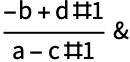
\includegraphics[scale=0.3]{images/introduction/O_2.png}
    \caption{The inverse of the pure function \(InverseFunction[(a # + b)/(c # + d) &]\) is rendered by the front end inside a WL notebook in the way it is reproduced here.}
    \label{fig:inversefunction}
\end{figure}